\documentclass[../nirs.tex]{subfiles}
\usepackage{pdflscape}

\begin{document}
\section{Построение концептуальной и физической модели данных}
Концептуальная модель данных определяет смысловую структуру рассматриваемой
системы [\ref{ref:wiki-er-диаграммы}]. С ее помощью можно представить рассматриваемую предметную область
множеством сущностей и связей между ними. Каждая сущность обладает набором
свойств, именуемых атрибутами. Основная задача концептуальной модели -- передать
фундаментальное принципы и основные функциональные возможности проектируемой
системы [\ref{ref:wiki-er-диаграммы}].

Любая информационная система включает в себя некоторую систему управления базами
данных (СУБД). Концептуальная модель представления данных не подходит для
создания таблиц в реляционной СУБД. Чтобы можно было создать реляционную базу
данных необходимо концептуальную модель перевести в логическую, а затем в
физическую  модель данных, предназначенную для конкретной СУБД. На рисунке
\ref{fig:3_1_db_logical} представлена логическая модель данных разрабатываемой
системы.

\clearpage
\begin{landscape}

\begin{figure}[H]
	\centering
	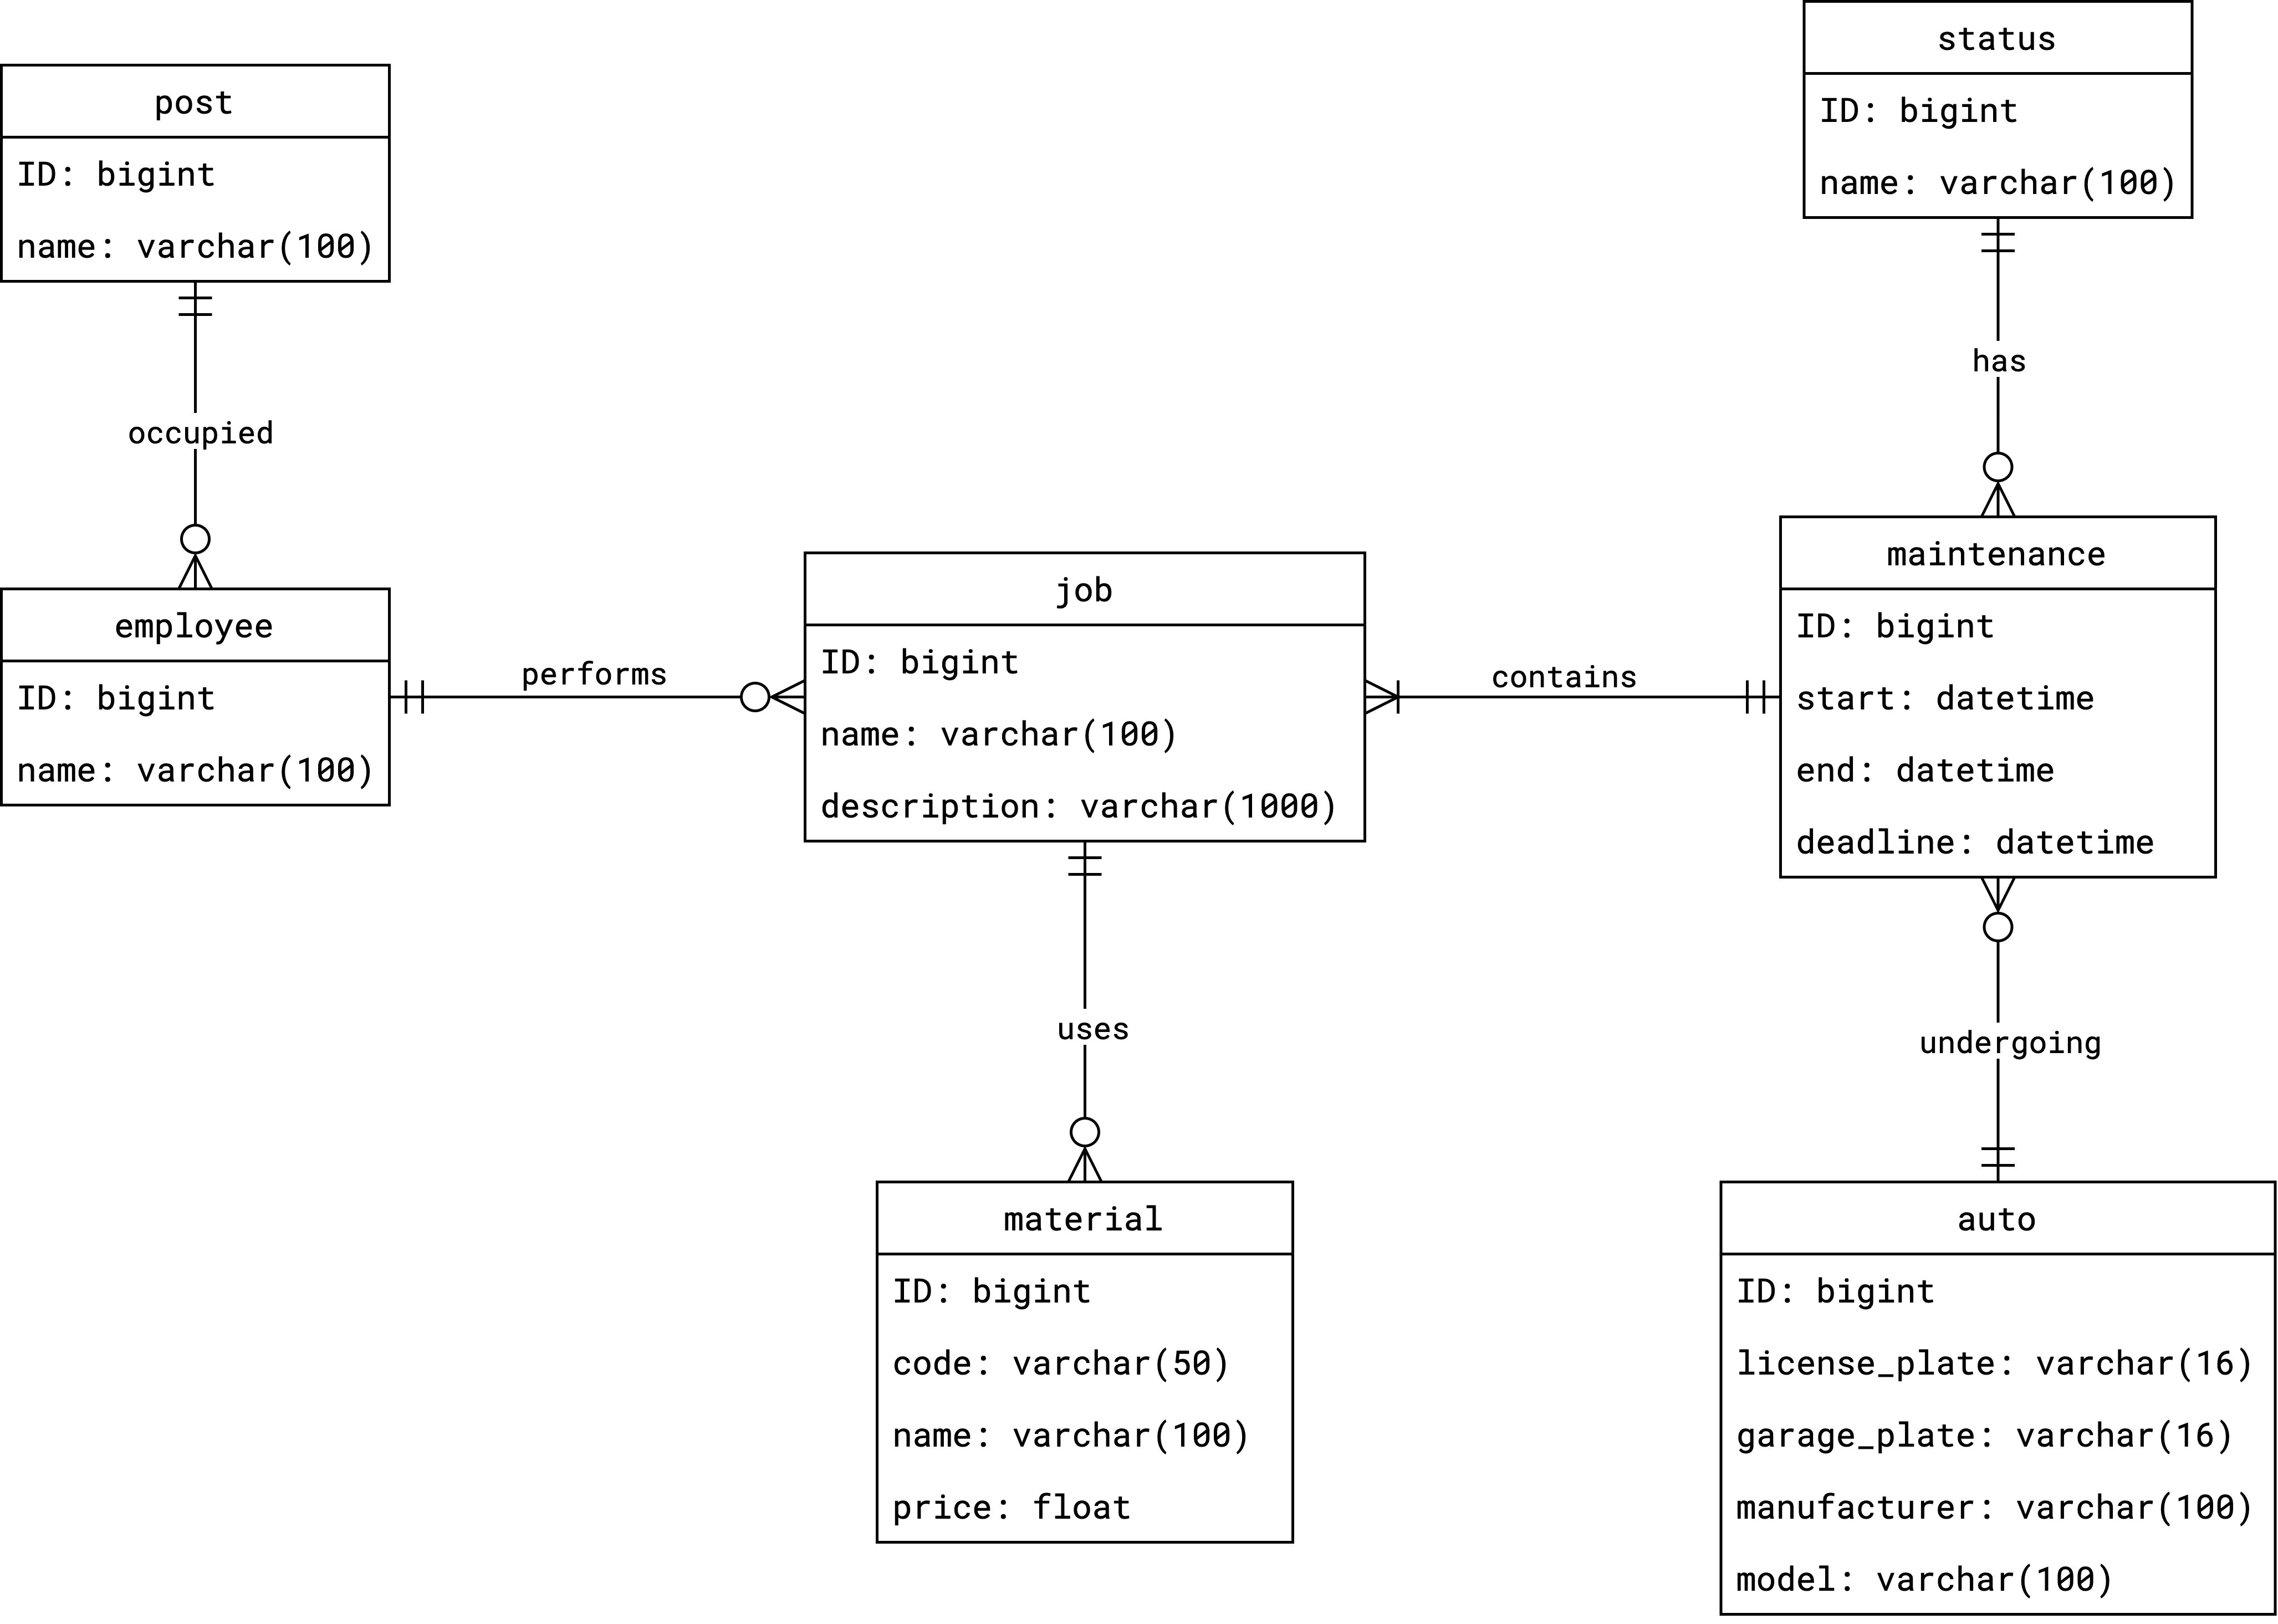
\includegraphics[keepaspectratio,width=\paperwidth]{./images/3_1_db_logical.png}
	\caption{Логическая модель данных разрабатываемой системы}
	\label{fig:3_1_db_logical}
\end{figure}

\end{landscape}
\clearpage

Спецификация сущностей приведена в таблицах \ref{tab:post} --
\ref{tab:auto}.
\begin{longtblr}
[
	caption = {Сущность \textquote{Должность} (post)},
	label = {tab:post},
]
{
	hlines, vlines,
	colspec = {L c c c},
	width = \textwidth,
	rowhead = 1,
	rowfoot = 0,
}
\SetCell[c=1,r=1]{c}{Код} & Тип & M & PK \\
    id & bigint & \checkmark & \checkmark \\
    name & varchar(100) & \checkmark &
\end{longtblr}

\begin{longtblr}
[
	caption = {Сущность \textquote{Сотрудник} (employee)},
	label = {tab:employee},
]
{
	hlines, vlines,
	colspec = {L c c c},
	width = \textwidth,
	rowhead = 1,
	rowfoot = 0,
}
\SetCell[c=1,r=1]{c}{Код} & Тип & M & PK \\
    id & bigint & \checkmark & \checkmark \\
    name & varchar(100) & \checkmark &
\end{longtblr}

\begin{longtblr}
[
	caption = {Сущность \textquote{Задание ТО} (job)},
	label = {tab:job},
]
{
	hlines, vlines,
	colspec = {L c c c},
	width = \textwidth,
	rowhead = 1,
	rowfoot = 0,
}
\SetCell[c=1,r=1]{c}{Код} & Тип & M & PK \\
    id & bigint & \checkmark & \checkmark \\
    name & varchar(100) & \checkmark & \\
    description & varchar(1000) & &
\end{longtblr}

\begin{longtblr}
[
	caption = {Сущность \textquote{Материал} (material)},
	label = {tab:material},
]
{
	hlines, vlines,
	colspec = {L c c c},
	width = \textwidth,
	rowhead = 1,
	rowfoot = 0,
}
\SetCell[c=1,r=1]{c}{Код} & Тип & M & PK \\
    id & bigint & \checkmark & \checkmark \\
    code & varchar(50) & \checkmark & \\
    name & varchar(100) & \checkmark & \\
    price & float & \checkmark &
\end{longtblr}

\begin{longtblr}
[
	caption = {Сущность \textquote{Статус} (status)},
	label = {tab:status},
]
{
	hlines, vlines,
	colspec = {L c c c},
	width = \textwidth,
	rowhead = 1,
	rowfoot = 0,
}
\SetCell[c=1,r=1]{c}{Код} & Тип & M & PK \\
    id & bigint & \checkmark & \checkmark \\
    name & varchar(100) & \checkmark &
\end{longtblr}

\begin{longtblr}
[
	caption = {Сущность \textquote{Техническое обслуживание} (maintenance)},
	label = {tab:maintenance},
]
{
	hlines, vlines,
	colspec = {L c c c},
	width = \textwidth,
	rowhead = 1,
	rowfoot = 0,
}
\SetCell[c=1,r=1]{c}{Код} & Тип & M & PK \\
    id & bigint & \checkmark & \checkmark \\
    start & datetime & \checkmark & \\
    deadline & datetime & \checkmark & \\
    end & datetime & \checkmark & \\
    mechanic\_id & bigint & \checkmark & \\
    auto\_id & bigint & \checkmark & \\
    status\_id & bigint & \checkmark & \\
\end{longtblr}

\begin{longtblr}
[
	caption = {Сущность \textquote{Автомобиль} (auto)},
	label = {tab:auto},
]
{
	hlines, vlines,
	colspec = {L c c c},
	width = \textwidth,
	rowhead = 1,
	rowfoot = 0,
}
\SetCell[c=1,r=1]{c}{Код} & Тип & M & PK \\
    id & bigint & \checkmark & \checkmark \\
    license\_plate & varchar(16) & \checkmark & \\
    garage\_plate & varchar(16) & \checkmark & \\
    manufacturer & varchar(100) & \checkmark & \\
    model & varchar(100) & \checkmark &
\end{longtblr}


\end{document}
